\begin{table}[htdp]
\caption[The Gram-Schmidt orthogonalization process]{The Gram-Schmidt orthogonalization process depicted for a set of two vectors. The input is the set of $u$ vectors on the left, the output are the orthonormal unit vectors $\hat{v}$ on the right. The vectors are plotted against the upper half of the unit circle to show the effect of dilations and contractions.}
\begin{center}
\begin{tabular}{ccc}
%
\raisebox{-0.5\height}{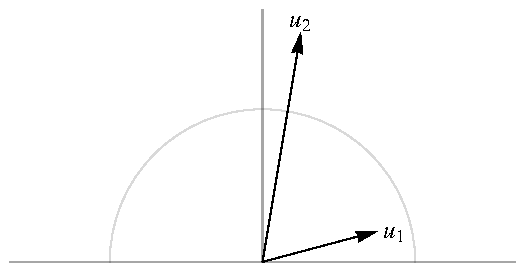
\includegraphics[ width = 2.25in ]{images/appendices/"gram schmidt"/gs_00.pdf}} &
%
$\Rightarrow$ &
%
\raisebox{-0.5\height}{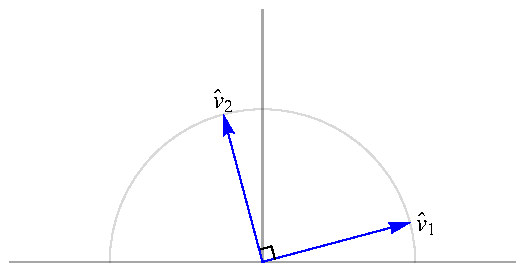
\includegraphics[ width = 2.25in ]{images/appendices/"gram schmidt"/gs_05.pdf}}
%
\end{tabular}
\end{center}
\label{tab:gs:io}
\end{table}


\endinput